\newcommand{\subgroup}{\le}
\newcommand{\subfield}{\le}
\newcommand{\isomorphism}{\simeq}

%Text Books : \cite{fraleigh}
%Module 1
%Direct products and finitely generated Abelian groups, fundamental theorem, Applications
%Factor groups, Fundamental homomorphism theorem, normal subgroups and inner automorphisms.
%Group action on a set, Isotropy subgroups, Applications of G- sets to counting.
%(Part II – Sections 11, 14, 16 & 17) (25 hours)
%Module 2
%Isomorphism theorems, Sylow theorems , Applications of the Sylow theory.
%(Part VII Sections 34, 36 & 37) (25 hours)
%Module 3
%Fermat’s and Euler Theorems, The field of quotients of an integral domain,
%Rings of polynomials, Factorisation of polynomials over a field.
%(Part IV – Sections 20, 21, 22 & 23) (20 hours)
%Module 4
%Non commutative examples, Homeomorphisms and factor rings, Prime and
%Maximal Ideals
%(Part V – Sections 24, 26 & 27) (20 hours)

%Module 1 - \cite{fraleigh} 11, (13), 14, (15), 16, 17
%Module 2 - \cite{fraleigh} 34, 36, 37
%Module 3 - \cite{fraleigh} 20, 21, 22, 23
%Module 4 - \cite{fraleigh} 24, 26, 27

%Advanced Abstract Algebra
%Module 1 - \cite{fraleigh} 29, 31, 32, 33
%Module 2 - \cite{fraleigh} 45, 46, 47
%Module 3 - \cite{fraleigh} 48, 49, 50
%Module 4 - \cite{fraleigh} 51, 53, 54, 55

%Missing - \cite{fraleigh} 1, 2, 3, 4, 5, 6, 7, 8, 9, 10,
%	12*, 13, 15, 18, 19, 25, 28, 30, 35, 38, 39, 40, 41, 42, 43, 44


\section{Introduction to Abstract Algebra}
%Week 01 Day 01 \S1-10
%\begin{story}
%\paragraph{`Abstract'}
%\footnote{There are many algebras. But, we are interested in the abstract notion 'algebra'.}
%Consider the collection of of all students in a class.
%A person can't be repeated in this collection so you might think this collection is always a set.
%But in this collection, there may be two with name starting with an `S'.
%Thus the collection of first letter of their names can give you the impression that some element is repeated.\\
%
%Thus, though the collection of students is a reality, set is an abstract idea which depends on the details we are interested in.
%And if a particular collection doesn't qualify to be a `set', we can't use set-theoretic results on it.
%(which is, everything below)
%\end{story}

\begin{definition}Set-theoretical foundation of Abstract Algebra
\begin{itemize}
	\item A \textbf{cartesian product}, $A \times B = \{ (a,b) \ : \ a \in A,\ b \in B \}$%\S0.4
	\item A \textbf{relation} on a set $A$ is a subset of $A \times A$.%\S0.7
	\item A \textbf{function} $f$ from $A$ into $B$,
	$f : A \to B$ is a relation such that \textit{every element of $A$ is related to some unique element of $B$} (well defined).%\S0.10
\end{itemize}
\end{definition}

\begin{definition} Functions :
	A \textbf{binary operation} on a set $A$ is a function $\ast : A \times A \to A$.%\S2.1
	%bi,tri,\dots are numerical prefixes with Latin origin.
	%di is a numerical prefix with Greek origin.
\end{definition}

``A binary operation on a set $A$ gives an algebra on $A$.''%\S1.0
\begin{story}
\paragraph{Abstract Algebra}
	It is the study of algebraic structures.
	We are interested in a few algebraic structures :
	\begin{enumerate*}
		\item Group
		\item Ring
		\item Integral Domain
		\item Field
	\end{enumerate*}
\end{story}

\begin{definition}
	A \textbf{binary algebraic structure} $<\!G,\ast\!>$ is a set $G$ together with a binary operation $\ast$.
\end{definition}

\begin{definition}[Group]
	A set $G$, closed under a binary relation $\ast$ satisfying the following three axioms -G1, G2, \& G3 is a group.%\S4.1
\begin{enumerate}[label=G\arabic*]
	\item Associativity \\
		For any three elements $a,b,c \in G,\ a \ast (b \ast c) = (a \ast b) \ast c$.
	\item Identity element\\
		There exists a unique element $e \in G$ such that $a \ast e = a = e \ast a$ for any element $a \in G$.
	\item Inverse elements\\
		For any element $a \in G$ there exists a unique element $a^{-1}$ such that $a \ast a^{-1} = e = a^{-1} \ast a$.
\end{enumerate}
\end{definition}

\begin{definition}Group terminologies :
\begin{itemize}
	\item A group is \textbf{abelian} if the binary operation is commutative. $a \ast b = b \ast a$%\S4.3
	\item The \textbf{order} of a group $G,\ast$ is the number of elements in $G$.%\S5.3
\end{itemize}
\end{definition}

\begin{definition}
	$\mathbb{Z}_n = \{ 0, 1, 2, \cdots, n-1 \}$
\end{definition}

\begin{remark}
	Consider $3,4 \in \mathbb{Z}_5$,
	$3 \ast 4 = 2 = 4 \ast 3$ since $7 \cong 2 \pmod 5$.
	$<\!\mathbb{Z}_5,+_5\!>$ is an abelian group of order 5.
\end{remark}

\begin{definition} Homomorphism \& Isomorphism
\begin{itemize}
	\item A function $\phi : A \to B$ is a \textbf{homomorphism} if for any two elements $x,y \in A$, $\phi (xy) = \phi(x)\phi(y)$%\S3.7
	\item A function $\phi : A \to B$ is an \textbf{isomorphism} if $\phi$ is a bijective, homomorphism.
	If two binary structures  are isomorphic, then they have the same (algebraic) structure.%\S3.7
\end{itemize}
\end{definition}

\begin{definition} Subgroup
\begin{itemize}
	\item A subset $H$ of a group $<\! G,\ast\! >$ is a \textbf{subgroup} of $G$ if $H$ is group with the same binary operation $\ast$.
	And is denoted by $H \subgroup G$.%\S5.4
	\item $G$ is the \textbf{improper} subgroup of $G$ and every other subgroup is \textbf{proper}.S5.5
	\item $\{e\}$ is the \textbf{trivial} subgroup of $G$ and every other subgroup is \textbf{non-trivial}.%\S5.5
	\item The \textbf{subgroup generated by} $g \in G$ is the subgroup $\{ g^n : n \in \mathbb{Z} \}$.%\S5.19
	\item The \textbf{order} of an element $g$ is order of the subgroup generated by $g$.%\S5.19
	\item An element $g \in G$ is a \textbf{generator} of $G$ if $g$ generates $G$.%\S5.19
	\item A group is \textbf{cyclic} if it has a generator.%\S5.19
\end{itemize}
\end{definition}

\begin{remark}
	Cyclic Groups :
\begin{itemize}
	\item Cyclic groups are abelian.%\S6.1
	\item Subgroups of cyclic groups are cyclic.%\S6.6
\end{itemize}
\end{remark}

\subsection{Some Proof Techniques}
\paragraph{Equality of two Sets}
$A = B \iff A \subset B$ and $B \subset A$\\
If $x \in A \implies x \in B$, then $A \subset B$
\paragraph{Uniqueness}
	Suppose there are two elements that qualify our conditions.
	We show (using the conditions) that they are the same, that is, unique.

	For example, $3 + a = \pi$.
	Suppose $a = x,y$.
	Then $3 + x = 3 + y \implies x = y$, provided that the values of $a$ comes from a set in which left cancelation law can be applied.
	Then $a$ is unique.

	Remember : We usually don't care to show what this unique element is.
	It may be also be the case that there is no such element, that is, proof of uniqueness doesn't imply existence.

\paragraph{Existence}
	There are constructive and non-constructive proofs for existence problems.
	Suppose we want to prove that $a\ast b$ has an inverse element.
	We know that $a,b$ has inverse elements $a^{-1},b^{-1}$.
	From those elements, we construct an element $b^{-1} \ast a^{-1}$ which is an inverse of $a \ast b$ by construction.

	And we may also prove existence without actually giving an object.
	Suppose we want to prove that $x^y \in \mathbb{Q}$ for some irrational numbers $x$ and $y$.
	We know that $\sqrt{2} \notin \mathbb{Q}$.
	Then, $\sqrt{2}^{\sqrt{2}}$ is either rational or irrational.
	Suppose it is irrational, then $\left(\sqrt{2}^{\sqrt{2}}\right)^{\sqrt{2}} = 2$ is rational.
	Thus the proof is complete, but we are yet to know whether $\sqrt{2}^{\sqrt{2}}$ is an irrational or rational.

%\pagebreak

%Week 01 Day 02 \S11.1-11
\section{Direct Products and Finitely Generated Abelian Groups}
\begin{definition}[Cartesian product of sets]
	Let $S_1,\ S_2, \cdots,\ S_n$ be a sets.
	Their cartesian product,
	\begin{equation}
		S_1 \times S_2 \times \cdots \times S_n = \prod_{i = 1}^n S_n = \{ (a_1,a_2,\cdots,a_n) :  a_i \in S_i \} 
	\end{equation}
	For example, $ \{A,B,C\} \times \{ 1,2 \} = \{ (A,1),(A,2),(B,1),(B,2),(C,1),(C,2) \}$.
\end{definition}

\begin{question}
	How many elements in $\mathbb{Z}_3 \times \mathbb{Z}_{10} \times \mathbb{Z}_9$ ?
\end{question}

\begin{theorem}[Direct product of Groups]
	Let $G_1,\ G_2,\ \cdots,\ G_n$ be groups.
	Then their cartesian product is a group with the binary operation $\ast$,
	\begin{equation}
		(a_1,\ a_2,\ \cdots,\ a_n) \ast (b_1,\ b_2,\ \cdots,\ b_n) = (a_1 \ast b_1,\ a_2 \ast b_2,\ \cdots,\ a_n \ast b_n)
	\end{equation}
	where the binary operation in  $a_i \ast b_i$ is the binary operation of the group $G_i$.
\end{theorem}
\begin{proof}
	$\prod\limits_{i = 1}^n G_i$ is a group if it satisfies the group axioms.
	\begin{enumerate}[label=G\arabic*]
		\item Associativity
			\begin{align*}
				(a_1,\ a_2,\ & \cdots,\ a_n) \big( (b_1,\ b_2,\ \cdots,\ b_n)(c_1,\ c_2,\ \cdots,\ c_n) \big) \\
				= & (a_1,\ a_2,\ \cdots,\ a_n)(b_1c_1,\ b_2c_2,\ \cdots,\ b_nc_n) \\
				= & \big( a_1(b_1c_1),\ a_2(b_2c_2),\ \cdots,\ a_n(b_nc_n) \big) \\
				= & \big( (a_1 b_1)c_1,\ (a_2b_2)c_2,\ \cdots,\ (a_nb_n )c_n \big) \\
				= &  (a_1b_1,\ a_2b_2,\ \cdots,\ a_nb_n)(c_1,\ c_2,\ \cdots,\ c_n) \\
				= & \big( (a_1,\ a_2,\ \cdots,\ a_n)(b_1,\ b_2,\ \cdots,\ b_n) \big)(c_1,\ c_2,\ \cdots,\ c_n)
			\end{align*}
		\item Existence of a unique identity element in $\prod\limits_{i = 1}^n G_i$\\
			Let $e_i$ be the identity element in $G_i$.
			Then $(e_1,\ e_2,\ \cdots,\ e_n)$ is the identity element in $\prod\limits_{i = 1}^n G_i$.
			\begin{align*}
				(a_1,\ a_2,\ \cdots,\ a_n)&(e_1,\ e_2,\ \cdots, e_n) \\
				& = (a_1e_1,\ a_2e_2,\ \cdots,\ a_ne_n) \\
				& = (a_1,\ a_2,\ \cdots,\ a_n)
			\end{align*}
		\item Existence of unique inverse element for each element in $\prod\limits_{i = 1}^n G_i$\\
			Let $(a_1,\ a_2,\ \cdots, a_n)$ be in $\prod\limits_{i = 1}^n G_i$.
			Then it has the inverse element $( a_1^{-1},\ a_2^{-1},\ \cdots,\ a_n^{-1} )$ in $\prod\limits_{i = 1}^n G_i$.
			\begin{align*}
				(a_1,\ a_2,\ \cdots a_n)&(a_1^{-1},\ a_2^{-1},\ \cdots, a_n^{-1}) \\
				& = (a_1a_1^{-1},\ a_2a_2^{-1},\ \cdots,\ a_na_n^{-1}) \\
				& = (e_1,\ e_2,\ \cdots,\ e_n)
			\end{align*}
	\end{enumerate}
\end{proof}

\begin{remark}
	We usually write $ab$ instead of $a \ast b$ and relevent binary operations are used in different contexts.
	Student should be able to recongnise the difference from the context.
\end{remark}

\begin{remark}
	$\mathbb{Z}_n = \{ 0,1,\cdots,(n-1) \}$ is a group with $+_n$.
	(addition modulo $n$)

	For example, Consider $(1,2) \in \mathbb{Z}_2 \times \mathbb{Z}_3$.
	We have, $(1,2) + (1,2) = (0,1)$ since $1 +_2 1=0$ and $2 +_3 2 = 1$.
\end{remark}

\begin{definition}
	Suppose all the groups $G_i$ are abelian.
	Then $\prod\limits_{i = 1}^n G_i$ is the direct sum of the groups $G_i$.
	And is represented by $\oplus_{i = 1}^n G_i$.
\end{definition}

\begin{theorem}
	$\mathbb{Z}_m \times \mathbb{Z}_n$ is cyclic and is isomorphic to $\mathbb{Z}_{mn}$ if and only if $m$ and $n$ are relatively prime.
\end{theorem}
\begin{proof}
	Sufficient part :
	Consider the cyclic subgroup\footnote{$(1,1) \in Z_m \times Z_n$.
	The cyclic group generated by $(1,1)$ has all its elements in $Z_m \times Z_n$.
	And therefore, it is a subgroup of $Z_m \times Z_n$} $H$ generated by $(1,1) \in \mathbb{Z}_m \times \mathbb{Z}_n$.
	It is enough to prove that the order of this cyclic subgroup $H$ is $mn$.
	The order of $H$ is the smallest power of $(1,1)$ that gives the identity $(0,0)$.
	The first component gives $0$ for multiples of $m$.
	And the second component gives $0$ for multiples of $n$.
	Since $m,n$ are relatively prime, $mn$ is the smallest power of $(1,1)$ that will give $(0,0)$.
	Thus $\mathbb{Z}_m \times \mathbb{Z}_n = H$ and is cyclic.
	\begin{important} Every cyclic group of order $mn$ is isomorphic to $\mathbb{Z}_{mn}$. Therefore, $\mathbb{Z}_m \times \mathbb{Z}_n \approx \mathbb{Z}_{mn}$.\end{important}

	Necessary part :
	Suppose $\gcd(m,n) = d > 1$.
	Then $mn/d$ is the smallest integer divisible by both $m$ and $n$.
	Consider $(r,s) \in \mathbb{Z}_m \times \mathbb{Z}_n$.
	$r$ gives $0$ in $mn/d$ since it is a multiple of $m$.
	Similarly, $s$ gives $0$ in $mn/d$ since it is a multiple of $n$.
	Thus, $\frac{mn}{d} (r,s) = (0,0)$.
	And the cyclic group generated by any element of $\mathbb{Z}_m \times \mathbb{Z}_n$ is a proper subgroup.
	Therefore $\mathbb{Z}_m \times \mathbb{Z}_n$ has no generators and it is not cyclic.
\end{proof}

\begin{corollary}
	$\prod\limits_{i = 1}^n \mathbb{Z}_{m_i}$ is cyclic and is isomorphic to $Z_{m_1m_2\cdots m_n}$ if and only if any two of the numbers $m_i$ are relatively prime.
\end{corollary}

\begin{question}
	Prove : For any non-negative integer $n$, there exists a cyclic group of order $n$, which is unique upto isomorphism.
\end{question}

\begin{theorem}
	Let $(a_1,\ a_2,\ \cdots,\ a_n) \in \prod\limits_{i = 1}^n G_i$. And $a_i$ are of finite order $r_i$ in $G_i$. Then the order of $\prod\limits_{i = 1}^n G_i$ is the least common multiple of $r_i$s.
\end{theorem}
\begin{proof}
	Least common multiple of $r_i$s is the smallest positive integer $d$ which is a multiple of all $r_i$s.
	For each $i$, the $r_i$th multiple of $a_i$ gives $0$ (identity).
	Thus, the order of the cyclic subgroup generated by $(a_1,\ a_2,\ \cdots,\ a_n)$ is the least common multiple of all the $r_i$s.
\end{proof}
\begin{remark}
	Consider $(3,6,12,16) \in \mathbb{Z}_4 \times \mathbb{Z}_{12} \times \mathbb{Z}_{20} \times \mathbb{Z}_{24}$.
	Order of $3 \in \mathbb{Z}_4$ is ${4}/{\gcd(3,4)} = 4$ ie, $<3> = \{ 3,2,1,0 \}$\\
	Order of $6 \in \mathbb{Z}_{12}$ is ${12}/{\gcd(6,12)} = 2$ ie, $<6> = \{ 6,0 \}$\\
	Order of $12 \in \mathbb{Z}_{20}$ is ${20}/{\gcd(12,20)} = 5$ ie, $<12> = \{ 12,4,16,8,0 \}$\\
	Order of $16 \in \mathbb{Z}_{24}$ is ${24}/{\gcd(16,24)} = 3$ ie, $<16> = \{ 16,8,0 \}$\\
	Order of $(3,6,12,16)$ is $lcm(4,2,5,3) = 2^2\ 3\ 5 = 60$.
\end{remark}

\begin{remark}
	Define $\overline{G_i} = \{ (e_1,\ e_2,\ \cdots,\ e_{i-1},\ a_i,\ e_{i+1},\ \cdots,\ e_n) : a_i \in G_i\}$.
	Then $G_i \approx \overline{G_i}$.
	And $\prod\limits_{i=1}^n G_i$ is the internal direct product of $\overline{G_i}$s.

	For example, $\mathbb{Z}_2 \times \mathbb{Z}_3 \approx \left( \mathbb{Z}_2 \times \{ 0 \} \right) \otimes \left( \{ 0 \} \times \mathbb{Z}_3 \right)$
\end{remark}

\begin{question}
	Internal direct product form of $\mathbb{Z}_{12} \times \mathbb{Z}_{60} \times \mathbb{Z}_{24}$ ?
\end{question}
%\pagebreak

%Week 01 Day 03 \S11.11-17
\section{Fundamental Theorem}
\begin{definition}
	A group $G$ is \textbf{finitely generated} if $G$ has a finite subset that generates $G$.
%	For example, $\{ 1,\rho^2,\mu,\mu\rho^2 \}$ is a finitely generated subgroup of $D_4$.
\end{definition}

\begin{theorem}[fundamental theorem of finitely generated abelian groups]
	Every finitely generated abelian group $G$ is isomorphic to a direct product of cyclic groups in the form
	\begin{equation}
		\mathbb{Z}_{{p_1}^{r_1}} \times\mathbb{Z}_{{p_2}^{r_2}} \times \cdots \times \mathbb{Z}_{{p_n}^{r_n}} \times \mathbb{Z} \times \mathbb{Z} \times \cdots \times \mathbb{Z}
	\end{equation}
	where $p_i$ are primes, not necessarily distict and $r_i$ are positive integers.
	The direct product is unique, except for the possible rearrangement of the factors.
\end{theorem}
\begin{proof}
	---proof is omitted---
\end{proof}

For example, $ G = \mathbb{Z}_{20} \times \mathbb{Z} \times \mathbb{Z}_{15} \times \mathbb{Z} \approx \mathbb{Z}_{2^2} \times \mathbb{Z}_3 \times \mathbb{Z}_5 \times \mathbb{Z}_5 \times \mathbb{Z} \times \mathbb{Z}$.
In the above case, Betti number of $G$ is $2$ (number of $\mathbb{Z}$ factors).
For any finite abelian group, Betti number is $0$.

\begin{remark}[finite abelian groups]
	Every finite group is finitely generated.
	And thus we can enumerate finite abelian group of any order.
\end{remark}

\begin{remark}
	There are precisely $6$ different abelian groups of order $360 = 2^3 3^2 5$.
	\begin{enumerate}
		\item $\mathbb{Z}_2 \times \mathbb{Z}_2 \times \mathbb{Z}_2 \times \mathbb{Z}_3 \times \mathbb{Z}_3 \times \mathbb{Z}_5$ 
		\item $\mathbb{Z}_2 \times \mathbb{Z}_{2^2} \times \mathbb{Z}_3 \times \mathbb{Z}_3 \times \mathbb{Z}_5$
		\item $\mathbb{Z}_{2^3} \times \mathbb{Z}_3 \times \mathbb{Z}_3 \times \mathbb{Z}_5$
		\item $\mathbb{Z}_2 \times \mathbb{Z}_2 \times \mathbb{Z}_2 \times \mathbb{Z}_{3^2} \times \mathbb{Z}_5$
		\item $\mathbb{Z}_2 \times \mathbb{Z}_{2^2} \times \mathbb{Z}_{3^2} \times \mathbb{Z}_5$
		\item $\mathbb{Z}_{2^3} \times \mathbb{Z}_{3^2} \times \mathbb{Z}_5$
	\end{enumerate}
\end{remark}

\begin{question}
	Group of order 360 with at least an element of order 8
\end{question}

\begin{definition}
	A group $G$ is \textbf{decomposible} if it is isomorphic to a direct product of two proper, non-trivial subgroups.
	Otherwise $G$ is \textbf{indecomposible}.
\end{definition}

	For example, $\mathbb{Z}_{2^3} \times \mathbb{Z}_3 \times \mathbb{Z}_3 \times \mathbb{Z}_5 \approx \mathbb{Z}_{24} \times \mathbb{Z}_{15}$ is decomposible.

\begin{remark}
	$G = \mathbb{Z}_2 \times \mathbb{Z}_2 \times \mathbb{Z}_2 \times \mathbb{Z}_{3} \times \mathbb{Z}_3 \times \mathbb{Z}_5 \approx \mathbb{Z}_2 \times \mathbb{Z}_{6} \times \mathbb{Z}_{30}$ is also decomposible.
	Since $G \approx (\mathbb{Z}_2 \times \mathbb{Z}_{6}) \times \mathbb{Z}_{30}$.
\end{remark}

\begin{theorem}
	The finite indecomposible abelian groups ar exactly the cyclic groups with order a power of a prime.
\end{theorem}
\begin{proof}
	Necessary part: 
	Let $G$ be a finite, indecomposible abelian group.
	By fundamental theorem of finitely generated abelian groups, $G$ is isomorphic to a direct product of cyclic groups of prime power order.
	$$ G \approx \mathbb{Z}_{{p_1}^{r_1}} \times \mathbb{Z}_{{p_2}^{r_2}} \times \cdots \times \mathbb{Z}_{{p_n}^{r_n}}$$
	Thus for $G$ to be indecomposible the direct product should be a cyclic group of prime power order.
	$G \approx \mathbb{Z}_{{p_1}^{r_1}}$.

	Sufficient part :
	Let $p$ be a prime and $r$ a non-negative integer.
	Cyclic group of order $p^r$ is isomorphic to $\mathbb{Z}_{p^r}$.
	Since every cyclic groups are abelian, $\mathbb{Z}_{p^r}$ is an abelian group of finite order $p^r$.
	It is enough to prove that $\mathbb{Z}_{p^r}$ is indecomposible.

	A proper, non-trivial subgroup of $\mathbb{Z}_{p^r}$ is of the form $\mathbb{Z}_{p^i}$ where $0 < i < r$.
	Suppose $\mathbb{Z}_{p^r}$ is decomposible.
	Then $\exists i,j \in \mathbb{Z}^+$ such that $\mathbb{Z}_{p^r} \approx \mathbb{Z}_{p^i} \times \mathbb{Z}_{p^j}$ and $i+j=r$.
	Clearly, $p^i$ and $p^j$ are not relatively prime, thus $\mathbb{Z}_{p^r} \not\approx \mathbb{Z}_{p^i} \times \mathbb{Z}_{p^j}$.
	Therefore, cyclic groups of order prime power are indecomposible.
\end{proof}

\begin{theorem}
	If $m$ divides the order of a finite abelian group $G$, then $G$ has a subgroup of order $m$.
\end{theorem}
\begin{proof}
	Let $G \approx \mathbb{Z}_{{p_1}^{r_1}} \times \mathbb{Z}_{{p_2}^{r_2}} \times \cdots \times \mathbb{Z}_{{p_n}^{r_n}}$.
	Then $|G| = p_1^{r_1} p_2^{r_2} \cdots p_n^{r_n}$.
	Suppose $m$ divides $|G|$, then $m = p_1^{s_1} p_2^{s_2} \cdots p_n^{s_n}$ where $0 \le s_i \le r_i$.
	Define $H = \mathbb{Z}_{{p_1}^{s_1}} \times \mathbb{Z}_{{p_2}^{s_2}} \times \cdots \times \mathbb{Z}_{{p_n}^{s_n}}$.
	Then $H$ is subgroup of order $m$.
\end{proof}

\begin{theorem}
	If $m$ is square-free integer, then every abelian group of order $m$ is cyclic.
\end{theorem}
\begin{proof}
	Let $m$ be a square-free integer and $G$ be an abelian group of order $m$.
	By fundamental theorem of finitely generated abelian groups
	$$ G \approx \mathbb{Z}_{{p_1}^{r_1}} \times \mathbb{Z}_{{p_2}^{r_2}} \times \cdots \times \mathbb{Z}_{{p_n}^{r_n}}$$
	We have, $m$ is square-free.
	Thus $r_i = 1$ and $p_i$ are distinct.
	Therefore, $G \approx \mathbb{Z}_{p_1 p_2 \cdots p_n}$ is a cyclic group of order $m$.
\end{proof}
%\pagebreak

%Week 01 Day 04 \S11E
\section{Exercises \S11}

\begin{question}
	Enumerate subgroups of $\mathbb{Z}_2 \times \mathbb{Z}_2 \times \mathbb{Z}_4$
\end{question}

\subsection{Abelian Groups}
\begin{remark}
Direct product of abelian groups is abelian.%\S11Ex46
\end{remark}

\begin{question}
	Enumerate abelian groups of order 72 ?
\end{question}

\begin{remark}
	Let $G$ be an abelian group.
	The subset $H$ of $G$ with identity element and all elements of order $n$ is subgroup of $G$ if and only if $n$ is a prime.%\S11Ex49
\end{remark}
\begin{proof}
	Suppose $a \in H$.
	Then every power of $a$ has order $n$.
	Suppose $n$ is not prime.
	Then $d$ divides $n$ and $a^d$ has order $n/d$.
\end{proof}

\subsection{Torsion Group and Torsion Coefficients}
\begin{remark}
If group $G$ is abelian, then its elements of finite order forms a subgroup.%\S11Ex39
(hint : $a,b \in G$ has finite order, then $ab$ has finite order. And $a \in G$ has finite order, then $a^{-1}$ has finite order)
\end{remark}
\begin{definition} 
	The \textbf{torsion group} of an abelian group $G$ is the subgroup of $G$ containing only those elements of finite order.%\S11Ex39
	An abelian group is \textbf{torsion free} if identity element is the only element of finite order.
	$G$ is Torsion free if Torsion group of $G$ is trivial, $\{ e \}$.%\S11Ex43
\end{definition}

\begin{definition}
	The integers $m_1,m_2,\cdots,m_n$ are torsion coefficients of $G$ such that $G \approx \mathbb{Z}_{m_1} \times \mathbb{Z}_{m_2} \times \cdots \times \mathbb{Z}_{m_n}$ where $m_i$ divides $m_{i+1}$.%\S11Ex44
\end{definition}

For example, $\mathbb{Z}_6 \times \mathbb{Z}_{12} \times \mathbb{Z}_{20}$ has torsion coefficients $2, 12, 60$

\begin{remark}[Algorithm to find torsion coefficients of a group] Suppose $G$ has a direct product form.%\S11Ex44c
	\begin{enumerate}[label=Step \arabic*]
		\item Find power of each prime in the direct product form
		\item List power of each prime
		\item Append 1s on left to make all lists to equal length
		\item Product of $i$th number on each list gives $m_i$
	\end{enumerate}
\end{remark}

For example, $G \approx \mathbb{Z}_6 \times \mathbb{Z}_{12} \times \mathbb{Z}_{20}$
\begin{enumerate}[label=Step \arabic*]
	\item $\mathbb{Z}_6 \times \mathbb{Z}_{12} \times \mathbb{Z}_{20} \approx \mathbb{Z}_2 \times \mathbb{Z}_3 \times \mathbb{Z}_{2^2} \times \mathbb{Z}_3 \times \mathbb{Z}_{2^2} \times \mathbb{Z}_5$
	\item (2,4,4), (3,3), (5)
	\item (2,4,4), (1,3,3), (1,1,5)
	\item (2,12,60)
\end{enumerate}

\subsection{Torsion $p$-subgroup}
\begin{commentary}
	``Caution : Torsion $p$-subgroup is a name suggested by 'Jacob'. And is not among the standard terminology in group theory.''
\end{commentary}

\begin{remark}
	Let $G$ be a group.
	Let $p$ be an integer, $(p > 1)$.
	Then the set of all element of $G$ of order $p$ together with the identity element is a group, if $p$ is a prime.
\end{remark}

For example :
Consider symmetric group, $S_3$.
It has three elements of order $2$, namely $\mu_1 = (2\ 3)$, $\mu_2 = (1\ 3)$ and $\mu_3 = (1\ 2)$.
Clearly, the set of all element of order $2$ together with identity $(\ )$ is not a subgroup of $S_3$ as $(1\ 2)(1\ 3) = (3\ 1\ 2)$ is an element of order $3$.
Thus by counter-example, for a prime $p$, the set of all elements of a non-abelian group $G$ together with identity is not necessarily a subgroup of $G$.

Let $G$ be an abelian group.
Let $p$ be a prime.
Let $H$ be the set of all element of $G$ of order $p$ together with the identity $e$.
Let $g,h \in H$.
Clearly, $g^p = e$ and $h^p = e$.
For every $g,h \in G,\ gh \in G$, since $G$ is abelian $(gh)^p = g^p h^p = e$.
Also we have, $g^{-1} = g^{p-1}$ is a element of order $p$.
Therefore, $H$ is a subgroup of $G$.

Let $g$ be an element of order $4$.
Then $g^2$ is a element of order $2$.
Thus, the subgroup generated by $g$ or the smallest subgroup containing $g$ has a element of order $2$.
Therefore, elements of order $4$ together with identity cannot be a subgroup of $G$.
Thus, `Torsion $p$-subgroup' exists only if $p$ is a square-free integer.

Let $g$ be an element of order $6$.
Then $g^2$ is an element of order $3$.
Again, elements of order $6$ together with identity cannot be a subgroup of $G$.
Thus, `Torsion $p$-subgroup' exists only if $p$ is a power of a prime. Thus, `Torsion $p$-subgroup' of $G$ exists only if $G$ is abelian and $p$ is a prime.

\subsection{Normal Factors of $G$}
This is a warm-up exercise for \S37.5, where the theory is discussed by Fraleigh. However, we are able to conclude the following :
\begin{remark}
	Let $G = H \times K$.
	Let $g \in G$. Then $g = (h,k) \in H \times K$.%\S11Ex50
	Clearly, $H$ is a subset of $G$, and  $H \times \{e\} \subgroup G$.
	This subgroup is isomorphic to $H$.
	Thus $h \in H$ suggests the existence of  $(h,e) \in G$.

	Similarly $k \in K$ suggests $(e,k) \in G$.
	Therefore, $hk \in G$ suggests $(h,e)(e,k) = (h,k) = (e,k)(h,e)$.
	We know that, $kh \in G$ suggest $(e,k)(h,e) \in G$.
	Thus, $hk = kh$ for every $h \in H$ and every $k \in K$.

	In other words, if $G = H \times K$, then $H,K$ are isomorphic to normal subgroups $H',K'$ of $G$ such that $H' \cap K' = \{ e \}$ and $G \isomorphism K \times H$.
\end{remark}
%\pagebreak

%Week 02 Day 01 \S13
\section{Cosets and Homomorphism}

\begin{definition}
	A \textbf{permutation group} $S_n$ is the set of all permutations on the set $\{1,2,\cdots,n\}$.	
\end{definition}

\begin{remark}
	Consider, $(1\ 2\ 3)(4\ 5), (1\ 2)(3\ 4) \in S_5$.
	\begin{commentary}
		I was wrong about the order in which the permuations are carried out. It follows the same order as function composition. That is, $f \circ g(x)$ implies $f(g(x))$. Similarly, $\sigma\rho$ implies $\sigma(\rho(1\ 2\ \dots\ n))$.
	\end{commentary}
	$$\begin{pmatrix} 1 & 2 \end{pmatrix} \begin{pmatrix} 3 & 4 \end{pmatrix} \ast \begin{pmatrix} 1 & 2 & 3 \end{pmatrix} \begin{pmatrix} 4 & 5 \end{pmatrix} =  \begin{pmatrix} 1 & 2 & 3 & 4 & 5 \\ 2 & 3 & 1 & 5 & 4 \\ 1 & 4 & 2 & 5 & 3 \end{pmatrix}  = \begin{pmatrix} 2 & 4 & 5 & 3 \end{pmatrix} $$
		$$\begin{pmatrix} 1 & 2 & 3 \end{pmatrix} \begin{pmatrix} 4 & 5 \end{pmatrix} \ast \begin{pmatrix} 1 & 2 \end{pmatrix} \begin{pmatrix} 3 & 4 \end{pmatrix} =  \begin{pmatrix} 1 & 2 & 3 & 4 & 5 \\ 2 & 1 & 4 & 3 & 5 \\ 3 & 2 & 5 & 1 & 4 \end{pmatrix}  = \begin{pmatrix} 1 & 3 & 5 & 4 \end{pmatrix} $$
	Clearly, $S_5$ is a non-abelian group of order 120.
\end{remark}

\begin{definition}
	Kernel of a function $\phi : G \to G'$ is the inverse image of the identity element in $G'$.%\S13.13
\end{definition}

\begin{definition}Cosets and Normal Subgroup,
\begin{itemize}
	\item A \textbf{left coset} $gH$ is the subset $\{ gh \in G : h \in H \}$ where $g \in G$ and  $H \subgroup G$.%\S10.2
	\item A \textbf{right coset} $Hg$ is the subset $\{ hg \in G : h \in H \}$ where $g \in G$ and  $H \subgroup G$.%\S10.2
	\item A subgroup $H$ of group $G$ is \textbf{normal} if $gH = Hg,\ \forall g \in G$.
	\item All subgroups of abelian groups are normal.
\end{itemize}
\end{definition}

\begin{remark}
	For example, $H = \{1,\rho^2,\mu,\mu\rho^2\}$ is a normal subgroup of $D_4$.
	And $K = \{1,\mu\}$ is a subgroup of $D_4$ which is not normal.
	Note that, $\rho\mu \ne \mu\rho$.
	Clearly, $\rho K \ne K\rho$.
	However, $\rho H = \{ \rho, \rho^3, \mu\rho^3, \mu\rho \} = H\rho$.
\end{remark}

\begin{remark}[Lagrange's Theorem]%\S10.10
	Let $G$ be a finite group.
	If $H \subgroup G$, then order of $H$ divides order of $G$.
\end{remark}
\begin{itemize}
	\item $aH \cap bH \ne \phi \implies aH = bH$.
	\item $\forall g \in G,\ g \in gH$.
	\item $\forall g \in G,\ |gH| = |H|$.
\end{itemize}

\begin{remark}[Cayley's Theorem]%\S8.16
	Every group is isomorphic to a group of isomorphisms.
\end{remark}

\begin{definition}
	Let $G,G'$ be groups.
	A \textbf{group homomorphism} is a function $\phi : G \to G'$ such that $\phi(x)\phi(y) = \phi(xy)$.
	Clearly $\phi(e) = e'$.
	A \textbf{trivial homomorphism} is a function $\phi : G \to G'$ such that $\phi(G) = \{ e' \}$.
\end{definition}


\begin{remark}
	Group homomorphism $\phi : G \to G'$ preserves identity, inverses and subgroups.
	And kernel of group homomorphism is a normal subgroup of $G$.%\S13.12
\end{remark}
\begin{remark}
	For example, $\phi : D_4 \to \mathbb{Z}_2$ defined by $\phi(\rho) = 1$ and $\phi(\mu) = 0$ is a group homomorphism with $\ker(\phi) = \{ 1,\rho^2,\mu,\mu\rho^2 \}$.
\end{remark}
%\pagebreak

%Week 02 Day 02 \S14.1-8
\section{Factor Groups}
\begin{remark}[factor group]
	Let $H$ be a normal subgroup of a group $G$.
	Then the \textbf{factor group} of $G$ over $H$, $G/H$ is the group of cosets of $H$ in $G$.
\end{remark}

\begin{remark}
	For example, $H = \{ 1,\rho^2,\mu,\mu\rho^2 \}$ is normal subgroup of $D_4$.
	And the factor group $D_4/H = \{ 1H,\rho H \}$.
\end{remark}

\begin{theorem}
	Let $\phi : G \to G'$ be a group homomorphism with kernel $H$.
	Then cosets of $H$ form a factor group, $G/H$ where $(aH)(bH) = (abH)$ Also, $\mu : G/H \to \phi[G]$ defined by $\mu(aH) = \phi(a)$ is an isomorphism.
\end{theorem}
\begin{proof}
	Let $\phi : G \to G'$ be a group homomorphism with $\ker(\phi) = H$.
	We have, $\phi^{-1}(\phi(a)) = \{ g \in G : \phi(g) = \phi(a) \}$.

	Let $x \in aH$.
	Then $x = ah$ for some $h \in H$.
	And $\phi(x) = \phi(ah) = \phi(a)\phi(h) = \phi(a)$, since $\phi(h) = e'$.
	Thus, $x \in \phi^{-1}(\phi(a))$ and $aH \subset \phi^{-1}(\phi(a))$.

	Let $x \in \phi^{-1}(\phi(a))$.
	Then $\phi(x) = \phi(a)$.
	And $\phi(a)^{-1} \phi(x) = e' \implies \phi(a^{-1}x) = e'$.
	Clearly, $a^{-1}x \in \ker(\phi)$.
	Thus, there exists $h \in H$ such that $a^{-1}x = h$.
	Therefore, $x = ah$ for some $h \in H$,.
	Thus, $x \in aH$ and $\phi^{-1}(\phi(a)) \subset aH$.
	Therefore, $\phi^{-1}(\phi(a)) = aH$.
	
	Similarly, $\phi^{-1}(\phi(a)) = Ha$.
	Thus $aH = Ha$ and $H$ is a normal subgroup of $G$.
	Therefore, we have the factor group $G/H$.

	To prove : $\mu : G/H \to \phi[G]$ is a one-one correspondence.
	ie, $aH \xleftrightarrow{\mu} \phi(a)$.
	To prove : $\mu$ is injective.
	Suppose $\mu(aH) = \mu(bH)$. Then $\phi(a) = \phi(b)$.
	And $b \in \phi^{-1}(\phi(a)) = aH$. Therefore, $bH = aH$.

	To prove : $\mu$ is surjective.
	Let $\phi(a) \in \phi[G]$.
	Then, there exists $aH$ such that  $\mu(aH) = \phi(a)$.

	We have, $\mu(aH) = \phi(a)$, $\mu(bH) = \phi(b)$, and $\mu((ab)H)  = \phi(ab)$.\\
	Therefore, $\mu((aH)(bH)) = \mu((ab)H) = \phi(ab) = \phi(a)\phi(b) = \mu(aH)\mu(bH)$.
	Thus $\mu$ is a homomorphism.
	Therefore $\mu$ is an isomorphism.
\end{proof}

\begin{theorem}
	Let $G$ be a group and $H \subgroup G$.
	Then left coset multiplication is well-defined by $(aH)(bH) = (ab)H$ if and only if $H$ is a normal subgroup of $G$.
\end{theorem}
\begin{proof}
	Necessary part :
	Suppose $(aH)(bH) = (ab)H$ is well-defined.
	Let $a \in G$.
	It is enough to prove that $aH = Ha$.
	Let $x \in aH$.
	Then $(xH)(a^{-1}H) = (xa^{-1})H$.
	Also $(aH)(a^{-1}H) = eH = H$.
	We have, coset multiplication is well-defined.
	Thus $xa^{-1} = h \in H \implies x = ha \in Ha$.
	Then, $aH \subset Ha$.
	Similarly, $Ha \subset aH$ and $aH = Ha$.
	Therefore, $H$ is a normal subgroup of $G$.

	Sufficient part:
	Suppose $H$ is a normal subgroup of $G$,
	and let $x \in aH$ and $y \in bH$.
	$x \in aH \implies x = ah_1$ for some $h_1 \in H$
	$y \in bH \implies y = bh_2$ for some $h_2 \in H$.
	Therefore $xy = (ah_1)(bh_2) = (a(h_1(bh_2)) = a((h_1b)h_2) = a((bh_3)h_2) = a(b(h_3h_2)) = a(bh_4)$.
	Since $H$ is a group, $h_3h_2 = h_4 \in H$
	Thus, $xy = a(bh_4) = (ab)h_4 \in (ab)H$ for all $x \in aH$ and $y \in bH$
	Thus $(aH)(bH) = (ab)H$.
\end{proof}

\begin{corollary}
	Let $H$ be a normal subgroup of $G$.
	Then the cosets of $H$ form a group $G/H$ under the binary operation $(aH)(bH) = (ab)H$.
\end{corollary}
\begin{proof}
	Let $H$ be a normal subgroup and $aH,bH,cH$ are cosets of $H$ in $G$.
	\begin{enumerate}[label=G\arabic*]
		\item Associativity\\
			$(aH)[(bH)(cH)] = (aH)[(bc)H] = [a(bc)]H = [(ab)c]H = [(ab)H](cH) = [(aH)(bH)](cH)$
		\item Existence of identity, $eH$\\
			$(aH)(eH) = (ae)H = aH$ and $(eH)(aH) = (ea)H = aH$.
		\item Existence of inverse $(a^{-1}H)$\\
			$(aH)(a^{-1}H) = (aa^{-1})H = eH$ and $(a^{-1}H)(aH) = (a^{-1}a)H = eH$.
	\end{enumerate}
\end{proof}

\begin{remark}
	$n\mathbb{Z}$ is a normal subgroup of $\mathbb{Z}$.
	And $\mathbb{Z}/n\mathbb{Z} \approx \mathbb{Z}_n$.
	$\mathbb{Z}_n$ is a torsion group isomorphic to a factor group of torsion free group $\mathbb{Z}$.
\end{remark}

\begin{remark}
	Let $c \in \mathbb{R}^*$.
	Then the cyclic group generated by $c$ is
	a normal subgroup of $\mathbb{R}$ and $\mathbb{R}/<c> \approx \mathbb{R}_c$.
\end{remark}

\begin{question}
	Let $c = 0.31$.
	Find the coset $x\ +<0.31>$ containing $2$.
\end{question}
%\pagebreak

%Week 02 Day 03 \S14.9-15
\section{Fundamental Homomorphism \& Automorphisms}
\subsection{Fundamental Homomorphism Theorem}
\begin{theorem}
	Let $H$ be a normal subgroup of $G$.
	Then $\gamma : G \to G/H$ is defined by
	$\gamma(x) = xH$  is a homomorphism with kernel $H$.
\end{theorem}
\begin{proof}
	$\gamma(x)\gamma(y) = (xH)(yH)$
	Let $h_1,h_2 \in H$, $(xh_1)(yh_2) = xyh_3h_2 = xyh_4$ for some $h_3,h_4 \in H$.
	Therefore $(xH)(yH) = (xy)H$.
	$\gamma(xy) = (xy)H = \gamma(x)\gamma(y)$.
	$\gamma(x) = xH = H \iff x \in H$.
	Therefore, $\ker(\gamma) = H$.
\end{proof}

\begin{remark}
	Suppose $H$ is a normal subgroup of a group $G$.
	Then, a homomorphism $\gamma : G \to G/H$ is a natural homomorphism.
\end{remark}

\begin{theorem}[Fundamental Homomorphism]
	Let $\phi : G \to G'$ be a group homomorphism with kernel $H$.
	Then $\phi[G]$ is a group, and $\mu : G/H \to \phi[G]$ given by $\mu(gH) = \phi(g)$ is an isomorphism.
	If $\gamma : G \to G/H$ is the homomorphism given by $\gamma(g) = gH$, then $\phi(g) = \mu\gamma(g)$ for each $g \in G$.
\end{theorem}
\begin{proof}
	$\mu$ is an isomorphism $G/H \xleftrightarrow{\mu}\phi[G]$.
	$\mu(\gamma(g)) = \mu(gH) = \phi(g)$.
	Thus $\mu\gamma = \phi$.
\end{proof}
\begin{commentary}
	``Every group homomorphism $\phi : G \to G'$ with kernel $N$ has a unique natural group homomorphism $\gamma : G \to G/N$ and a unique isomorphism $\mu : G/N \to G'$ such that $\phi = \mu\gamma$. That is, $\phi(g) = \mu(\gamma(g)) = \mu(gN)$.''
\end{commentary}

\subsection{Inner Automorphism}
\begin{theorem}
	Let $H$ be a subgroup of $G$, then the following statements are equivalent:
	\begin{enumerate}
		\item $ghg^{-1} \in H,\ \forall g \in G,\ h \in H$
		\item $gHg^{-1} = H,\ \forall g \in G$
		\item $gH = Hg,\ \forall g \in G$
	\end{enumerate}
\end{theorem}
\begin{proof}
	Let $G$ be a group and $H \subgroup G$.
	By right multiplication,  $gHg^{-1} = H \iff gH = Hg$
	Trivially, $\forall h \in H,\ ghg^{-1} \in H \iff gHg^{-1} \subset H$
	Therefore, it is enough to prove that $H \subset gHg^{-1}$
	Let $h \in H$ and $x \in G$, then $xhx^{-1} = h'$ for some $h' \in H$.
	Then $h = x^{-1}h'x = x^{-1}h'(x^{-1})^{-1} \in gHg^{-1}$ where $x^{-1} = g \in G$.
	Thus $h \in gHg^{-1}$ and $H \subset gHg^{-1}$.
	Therefore $gHg^{-1} = H$.
\end{proof}

\begin{definition}Automorphisms : 
\begin{itemize}
	\item An \textbf{automorphism} of $G$ is an isomorphism $\phi : G \to G$
	\item The \textbf{inner automorphism} of $G$ by $g \in G$ is the isomorphism\\
	$i_g : G \to G$ defined by $i_g(x) = gxg^{-1}$ for all $x \in G$
	\item The \textbf{conjugate} of $x$ by $g$ is the element $gxg^{-1} \in G$
	\item The \textbf{conjugate subgroup} of subgroup $H$, $i_g[H] = \{ ghg^{-1} : h \in H \}$
\end{itemize}
\end{definition}

\begin{remark}
	For example, $i_\rho : D_4 \to D_4$ defined by $i_\rho(x) = \rho x \rho^{-1}$ is an inner automorphism.
	We have, $H = \{ 1,\mu \}$ is a subgroup of $D_4$.
	The conjugate subgroup $i_\rho[H] = \{ 1,\mu\rho^2 \}$.
\end{remark}

\begin{remark}
	Normal subgroups are invariant under any inner automorphism.
\end{remark}
%\pagebreak

%Week 02 Day 04 \S14E
\section{Exercise \S14}
\subsection{Normal subgroups}
\begin{question}
	Prove that the notion of normality is stronger than abelian. %S14E23b
\end{question}

\begin{remark}
	Let $G$ be a group. Then intersection of normal subgroups of $G$ is a normal subgroup of $G$.%\S14E31
\end{remark}
\begin{proof}
	Let $\mathcal{N}$ be a nonempty subfamily of normal subgroups of $G$. Let $N$ be the intersection of subgroups in $\mathcal{N}$. Clearly, intersection of subgroups of $G$ is also subgroup of $G$. 

	Suppose $x \in N$. Then $x \in H$ for every $H \in \mathcal{N}$. Suppose $x \in N$. Then $gxg^{-1} \in H$, for every normal subgroup $H \in \mathcal{N}$. Thus $gxg^{-1} \in N$. Therefore, $N$ is a normal subgroup of $G$.
\end{proof}

\begin{challenge}
	Let $\phi : G \to G'$ and $\psi : G \to G'$ be two group homomorphism with kernel $H$ and $K$ respectively. Show that $\phi\psi : G \to G'$ defined by $\phi\psi(g) = \phi(g)\psi(g)$ is also a group homomorphism, but $\ker(\phi\psi) \ne H \cap K$.\\
	\textit{(hint : Construct $\psi$ such that $\phi(g)\psi(g) = e$ for some $g \notin H$)}
\end{challenge}

\begin{remark}
	Let $S \subset G$, then $G$ has a smallest, normal subgroup containing $S$.%\S14E32
	\end{remark}
\begin{proof}
	Let $N$ be the intersection of all normal subgroups of $G$ containing $S$. Then $S \subset N$ and $N$ is a normal subgroup of $G$. Let $H$ be the smallest, normal subgroup of $G$ containing $S$. Then $N \subset H$. Therefore, $H = N$.
\end{proof}

\begin{remark}
	If a finite group $G$ has exactly one subgroup $H$ of order $m$, then $H$ is normal.%\S14E34
\end{remark}
\begin{proof}
	Let $G$ be a finite group. Suppose $G$ has only one subgroup of order $m$, say $H$. We know that, conjugate of a subgroup is a subgroup of same order. Thus, conjugates of $H$ are $H$ itself. Thus, $xHx^{-1} = H$ for every $x \in G$. Therefore, $xH = Hx$ for every $x \in G$ and $H$ is a normal subgroup of $G$.
\end{proof}

\begin{remark}
	If $G$ has a subgroup of order $s$, then the intersection of all subgroups of order $s$ is a normal subgroup of $G$.%\S14E36
\end{remark}
\begin{proof}
	Let $G$ be a group. Let $H$ be a subgroup of $G$ of order $s$. Let $N$ be the intersection of all subgroups of $G$ of order $s$. ??
\end{proof}

\subsection{Linear Groups}
\begin{definition}
	The set of all $n \times n$, non-singular matrices with real entries is a group under matrix multiplication. This group is the \textbf{General Linear Group} and is denoted by $GL(n,\mathbb{R})$.
\end{definition}

\begin{definition}
	The set of all $n \times n$ matrices with real entries and determinant $\pm 1$ is a group under matrix multiplication. This group is the \textbf{Special Linear Group} and is denoted by $SL(n,\mathbb{R})$.
\end{definition}

\begin{remark}
	$SL(n,\mathbb{R})$ is a normal subgroup of $GL(n,\mathbb{R})$%\S14E40
\end{remark}
\begin{proof}
	Let $A \in GL(n,\mathbb{R})$ and $B \in SL(n,\mathbb{R})$. Let $r = |A|$ and we have $|B| = \pm 1$. Then $|AB| = |A|\ |B| = \pm r$.

	Let $M_r$ be the set of all matrices with determinant $\pm r$ where $r \in \mathbb{R}$. Clearly, for every matrix $A$ with determinant $r$, $A \in M_r$. And there exists a matrix $C = B^{-1}AB$. Then, $|C| = |B^{-1}|\ |A|\ |B| = \pm r$. Thus, $C \in M_r$ and $AB = BC$. Clearly, $M_r$ is a left coset of $GL(n,\mathbb{R})$. Therefore, $SL(n,\mathbb{R})$ is a normal subgroup of $GL(n,\mathbb{R})$.
\end{proof}

\subsection{Factor Group}
\begin{remark}
	$A_n$ is a normal subgroup of $S_n$.
	And $S_n/A_n \isomorphism \mathbb{Z}_2$.%\S14E24
\end{remark}
\begin{proof}
	Let function $\phi : S_n \to \mathbb{Z}_2$ be defined by $\phi(\sigma) = 0$ if $\sigma$ is an even permutation and $\phi(\sigma) = 1$ if $\sigma$ is an odd permutation. Then $\phi$ is a homomorphism with kernel $A_n$, the set of all even permutations in $S_n$. We know that, the kernel of a homomorphism is a normal subgroup of the domain. Therefore, $A_n$ is a normal subgroup of $S_n$.
\end{proof}

\begin{remark}
	If $H$ is normal subgroup of $G$ and $(G:H) = m$, then $a^m \in H$ for all $a \in G$.%\S14E30
\end{remark}
\begin{proof}
	Let $H$ be a normal subgroup of $G$ such that $(G:H) = m$. Then $|G/H| = m$. Let $a \in G$, then $aH \in G/H$. Then by Lagrange's theorem, order of $aH$ divides $m$. Therefore, $(aH)^m = eH$. We have, $(aH)^m = a^mH$. Therefore, $a^m \in H$.
\end{proof}

\begin{remark}
	Every factor group of an abelian group is also abelian.%\S14E23gh
\end{remark}
\begin{proof}
	Let $G$ be an abelian group and $H$ be a normal subgroup of $G$. Then $G/H$ is a factor group of $G$. Let $aH, bH \in G/H$. Then, $(aH)(bH) = (ab)H = (ba)H = (bH)(aH)$. Clearly, factor group of an abelian group is abelian.
\end{proof}

\begin{remark}
	Let $G$ be a group and  $T$ be the torsion subgroup of $G$, then the factor group, $G/T$ is torsion free.%\S14E26
\end{remark}
\begin{proof}
	Let $G$ be a group $T$ its torsion subgroup. Let $g \in G$. If the order of $g$ is finite, then $g \in T$. Suppose $G/T$ has a element of finite order $m > 1$, say $xT$ where $x \notin T$. Then $x$ is an element of infinite order.

	We have, order of $xT$ is $m$. That is, $(xT)^m = eT$. Thus, $(xT)^m = (x^m)T = eT$. Therefore, $x^m  = y \in T$. Since $y \in T$, $y$ is an element of finite order, say $r$. Then $(x^m)^r = x^{mr} = e$. This is a contradiction as $x$ is an element of infinite order. Therefore, every element of $G/T$ except $eT$ are of infintie order. Clearly, $G/T$ is torsion free.
\end{proof}

\subsection{Commutator subgroup}
\begin{definition}
	A \textbf{commutator} $c$ in group $G$ is an element in the form $c = aba^{-1}b^{-1}$ for some $a,b \in G$.
	The \textbf{commutator subgroup} is the smallest normal subgroup containing all commutators in $G$.
\end{definition}

\begin{remark}
	Let $C$ be the commutator subgroup of $G$, then $G/C$ is abelian.%\S14E33
\end{remark}
\begin{proof}
	Let $C$ be the commutator subgroup of $G$. Let $x,y \in G$. Then $x^{-1}yxy^{-1} \in C$. Therefore, $x(x^{-1}yxy^{-1}) \in xC$ and $y(x^{-1}yxy^{-1}) \in yC$. But, $x(x^{-1}yxy^{-1})y(x^{-1}yxy^{-1}) = yx(x^{-1}yxy^{-1}) \in (yx)C$. Therefore, $(xC)(yC) = (yx)C = (yC)(xC)$. Clearly, $G/C$ is abelian.
\end{proof}

\begin{remark}
	The factor group $G/C$ is the abelianised version of $G$.
\end{remark}

\begin{remark}
	Let $G$ be a group and $C$ be the commutator group of $G$. Let $H$ be a normal subgroup of $G$. If $G/H$ is abelian, then $C$ is a subgroup of $H$.
\end{remark}

\begin{question}
	Find commutator subgroup of the dihedral group $D_4$ ?
\end{question}

\subsection{Automorphism}
\begin{remark}
	Every inner automorphism is an identity map for an abelian group. %\S14E23c
\end{remark}
\begin{proof}
	Let $G$ be an abelian group and $g \in G$. Then $i_g : G \to G$ is defined by $i_g(x) = gxg^{-1} = gg^{-1}x = x$. Clearly, $i_g$ is an identity map.
\end{proof}

\begin{remark}
	Set of all $g \in G$ such that the inner automorpism $i_g$ is an identity map is normal.%\S14E38
\end{remark}
\begin{proof}
	Let $H$ be the set of all $g \in G$ such that $i_g$ is an identity map.
	\begin{align*}
		H & = \{ g \in G : i_g(x) = x,\ \forall x \in G\} \\
		& = \{ g \in G : gxg^{-1} = x,\ \forall x \in G\}\\
		& = \{ g \in G : gx = xg,\ \forall x \in G \}
	\end{align*}
	Therefore, $H$ is a normal subgroup of $G$.
\end{proof}
\begin{remark}
	Set of automorphisms $\Gamma$ of a group $G$ is a group under composition. And the set of inner automorphisms is a normal subgroup of $\Gamma$.
\end{remark}
\begin{proof}
	Let $G$ be a group. We know that, the composition of two automorphisms is also an automorphism. Also, the composition of functions is associative. Let $i$ be the identity map and $\mu$ be any automorphism. Then $i\mu = \mu = \mu i$. Since automorphisms are bijective, there exists a unique inverse $\mu^{-1}$ for each automorphism $\mu$ such that $\mu\mu^{-1} = i$. Clearly, the set of all automorphisms of a group $G$ is also a group.
\end{proof}

\begin{remark}
	Subgroup conjugacy is an equivalance relation on the set of subgroups.%\S14E27
\end{remark}
\begin{proof}
	Let $H$ be a subgroup of a group $G$. Conjugation is reflexive, since $eHe^{-1} = H$ and $H \sim H$. 
	
	Let $K$ be a conjugate subgroup of $H$. That is, $H \sim K$. Then $K = gHg^{-1}$. Clearly, $H = g^{-1}K(g^{-1})^{-1}$. Thus, $H$ is a conjugate of $K$. ie, $K \sim H$.

	Let $H \sim K$ and $K \sim L$. Then we have $x,y \in G$ such that $K = xHx^{-1}$ and $L = yKy^{-1}$. Now, $L = y(xHx^{-1})y^{-1} = (yx)H(yx)^{-1}$. Thus, $H \sim L$. 
\end{proof}

\begin{question}
	Find the automorphism group $\Gamma(\mathbb{Z}_2 \times \mathbb{Z}_4)$ ?
\end{question}
%\pagebreak

%Week 03 Day 01 \S15
\section{Simple Groups}
\begin{remark}Factor Group Computations :
\begin{itemize}
	\item The converse of Lagrange's theorem is false.\\
	For example, $A_4$ has order $12$, but doesn't have a subgroup of order $6$.
	\item Factor group of a cyclic group is cyclic.\\
	(hint : if $g$ is a generator of $G$, then $gH$ is a generator of $G/H$.)
\end{itemize}
\end{remark}

\begin{question}
	Show that $\mathbb{Z}_4 \times \mathbb{Z}_6 / <(2,3)> \approx \mathbb{Z}_4 \times \mathbb{Z}_3$.
\end{question}

\begin{definition}
	A group is simple if it is non-trivial and has no proper, non-trivial normal subgroups.
\end{definition}

\begin{remark}
	Abelian, simple groups are $\mathbb{Z}_p$, the cyclic groups of prime order.
\end{remark}

\begin{remark}
	Symmetric group, $S_3$ is not simple.\\
	The subgroup, $\{ \rho_0,\rho_1,\rho_2\}$ is a normal subgroup of $S_3$.
\end{remark}

\begin{remark}
	Smallest nonabelian, simple group is $A_5$.\\
	Every nonabelian, simple group of order $60$ is isomorphic to $A_5$.
\end{remark}


\begin{remark} Simple groups :
\begin{itemize}
	\item Alternating groups $A_n$ are simple for $n \ge 5$.%\S15.15
	\item Every finite group can be factorised into simple groups.%\S15.15
	\item Every finite, non-abelian, simple group is of even order.%\S15.15
	\item Group homomorphism preserves normal subgroups.%\S15.16
	\item $M$ is maximal normal subgroup of $G$ if and only if $G/M$ is simple.%\S15.18
	\item Center $Z(G) = \{ z \in G : zg = gz,\ \forall g \in G \}$ is normal.%\S15.19
	\item Center of non-abelian groups of order $pq$ are trivial if $p,q$ are primes.%\S15.19
	\item Factor group, $G/N$ is abelian if and only if $C$ is a subgroup of $N$.%\S15.20
\end{itemize}
\end{remark}

\begin{question}
	$G$ is simple and $H$ is subgroup of $G$, then $H$ is simple ?
\end{question}

%\pagebreak

%Week 03 Day 02 \S16.1-10
\section{Group Action on a Set}
\begin{definition}%\S16.1
	An action of a group $G$ on a set $X$ is a map.
	$\ast : G \times X \to X$ such that
	\begin{enumerate}
		\item $ex = x,\ \forall x \in X$
		\item $(g_1g_2)(x) = g_1(g_2x),\ \forall x \in X,\ \forall g_1,g_2 \in G$
	\end{enumerate}
	Then $X$ is a $G$-set.
\end{definition}

\begin{theorem}
	Let $X$ be a $G$-set.
	$\forall g \in G,\ \sigma_g : X \to X$ defined by $\sigma_g(x) = gx$ is a permutation of $X$.
	Also, the map $\phi : G \to S_X$ defined by $\phi(g) = \sigma_g$ is a homomorphism with the property that $\phi(g)(x) = gx$.
\end{theorem}
\begin{proof}
	Suppose $X$ is a $G$-set.
	Let $g \in G$, and $x_1,x_2 \in X$.

	Suppose $\sigma_g(x_1) = \sigma_g(x_2)$. $\implies gx_1 = gx_2 \implies g^{-1}(gx_1) = g^{-1}(gx_2) \implies (g^{-1}g)x_1 = (g^{-1}g)x_2$. $\implies ex_1 = ex_2 \implies x_1 = x_2$. Thus, $\sigma_g$ is injective.

	Let $x \in X$. Then $\sigma_g(g^{-1}x) = g(g^{-1}x) = (gg^{-1})x = ex = x$. Thus, $\sigma_g$ is surjective. Therefore, $\sigma_g$ is a permutation of $X$, $\sigma_g \in S_X$.

	Let $g_1,g_2 \in G$.
	And $\phi(g_1)(x) = \sigma_{g_1}(x) = g_1x$, $\phi(g_2)(x) = \sigma_{g_2}(x) = g_2x$.
	$\phi(g_1g_2)(x) = \sigma_{g_1g_2}(x) = (g_1g_2)x = g_1(g_2x) = \sigma_{g_1}(g_2x) = \phi(g_1)(g_2x) = \phi(g_1)(\sigma_{g_2}(x)) = \phi(g_1)(\phi(g_2)(x)) = \phi(g_1)\phi(g_2)(x)$.
	Therefore, $\phi(g_1g_2) = \phi(g_1)\phi(g_2)$ and $\phi$ is a homomorphism.
\end{proof}

\begin{definition}Group Action,
\begin{itemize}
	\item $G$ acts \textbf{faithfully} on $X$, if $e$ is the only element that leaves every $x \in X$ fixed. 
	\item $G$ is \textbf{transitive} on $X$ if for every $x_1,x_2 \in X,\ \exists g \in G$ such that $gx_1 = x_2$.
	$G$ is transitive on $X$ iff the subgroup $\phi[G]$ of $S_X$ is transitive.
\end{itemize}
\end{definition}
%\pagebreak

%Week 03 Day 03 \S16.11-17
\section{Isotropy subgroups \& Orbits}
\begin{definition}Let $X$ be a $G$-set.
\begin{itemize}
	\item The subset fixed by $g$, $X_g = \{ x \in X : gx = x \}$
	\item The isotropy subgroup of $x$, $G_x = \{ g \in G : gx = x \}$\\
		Let $Y \subset X$, then $G_Y = \{ g \in G : gy = y, \forall y \in Y \}$ is a subgroup of $G$. %\S16E12
	\item The orbit of $x$ in $X$ under $G$, $Gx = \{ gx \in X : g \in G \}$
\end{itemize}
\end{definition}

\begin{theorem}
	Let $X$ be a $G$-set.
	Then $G_x$ is a subgroup of $G$, $\forall x \in X$.
\end{theorem}
\begin{proof}
	Let $x \in X$.
	And $g_1, g_2 \in G_x$.
	Then $g_1x = x$ and $g_2x = x$.

	Clearly, $(g_1g_2)x = g_1(g_2x) = g_1x = x$.
	Therefore, $g_1g_x \in G_x$.
	Also $ex = x \implies e \in G_x$.
	Let $g \in G_x$.
	Then $gx = x \implies g^{-1}(gx) = g^{-1}x \implies (g^{-1}g)x = g^{-1}x \implies x = g^{-1}x$.
	Thus, for any $g \in G_x$, $g^{-1} \in G_x$.
	Therefore, $G_x$ is a subgroup of $G$ for any $x \in X$.
\end{proof}

\begin{theorem}
	Let $X$ be a $G$-set and $x_1,x_2 \in X$.
	Then the relation $\sim$ defined by $x_1 \sim x_2$ iff $gx_1 = x_2$ is an equivalence relation.
\end{theorem}
\begin{proof}
	Let $x \in X$.
	Then $ex = x \implies x \sim x$.
	Let $x_1, x_2 \in X$ and $x_1 \sim x_2$.
	Then there exists some $g \in G$ such that $gx_1 = x_2$.
	We have, $g^{-1}x_2 = g^{-1}(gx_1) = (g^{-1}g)x_1 = ex_1 = x_1$.
	Therefore, $x_2 \sim x_1$.
	Let $x_1,x_2,x_3 \in X$ and $x_1 \sim x_2$ and $x_2 \sim x_3$.
	Then there are $g_1,g_2 \in G$ such that $g_1x_1 = x_2$ and $g_2x_2 = x_3$.
	Clearly, $g_2g_1 \in G$ and $(g_2g_1)x_1 = g_2(g_1x_1) = g_2x_2 = x_3$.
	Therefore, $x_1 \sim x_3$.
\end{proof}

\begin{theorem}
	Let $X$ be a $G$-set and $x \in X$.
	Then $|Gx| = (G:G_x)$.
	If $|G|$ is finite, then $|Gx|$ is a divisor of $|G|$.
\end{theorem}
\begin{proof}
	We have $Gx$ is the orbit of $x$ in $X$ under $G$ and ${L_G}_x$ is the left cosets of $G_x$ in $G$.
	Let $x_1 \in Gx$.
	Then there exists $g_1 \in G$ such that $x_1 = g_1x$.
	Define $\psi : Gx \to {L_G}_x$ by $\psi(x_1) = g_1G_x$.\\
	Step 1 : $\psi$ is well-defined.

	Let $x_1 \in Gx$. Suppose there exists $g_1,g_1' \in G$ such that $g_1x = x_1$ and $g_1'x = x_1$.
	Then we have, $g_1x = g_1'x \implies x = g_1^{-1}(g_1'x) = (g_1^{-1}g_1')x$.
	Thus, $g_1^{-1}g_1' \in G_x$.
	Therefore, $g_1(g_1^{-1}g_1') \in g_1G_x$.
	Clearly, $g_1(g_1^{-1}g_1') = (g_1g_1^{-1})g_1' = g_1' \in g_1G_x$.
	Therefore, $g_1G_x = g_1'G_x$.
	And $\psi(x_1) = g_1G_x$ is well-defined.\\
	Step 2 : $\psi$ is one-to-one.

	Suppose $\psi(x_1) = \psi(x_2)$.
	Let $x_1, x_2 \in Gx$ such that $x_1 = g_1x$ and $x_2 = g_2x$.
	Then we have $\psi(x_1) = \psi(x_2) \implies g_1G_x = g_2G_x$.
	Thus, $g_2 = g_1g$ for some $g \in G_x$.
	Clearly, $x_2 = g_2x = (g_1g)x = g_1(gx) = g_1x = x_1$.	\\
	Step 3 : $\psi$ is onto.

	Let $g_1G_x$ be a left coset of $G_x$ in $G$.
	Then we have, $g_1 \in G$ and $g_1x \in Gx$, say $x_1$.
	Therefore, there exists $x_1 \in Gx$ such that $\psi(x_1) = g_1G_x$.
\end{proof}

%\pagebreak

%Week 03 Day 04 \S16E
\section{Exercise \S16}
\begin{definition}
	Let $X$ be a $G$-set. And $S \subset X$. Then $S$ is a \textbf{sub-$G$-set} if the orbit $Gs$ of each $s \in S$ is contained in $S$.
	\begin{equation}
		S = \bigcup_{s \in S} Gs
	\end{equation}
\end{definition}

\begin{remark}
\begin{itemize}
	\item Every $G$-set is a union of its orbits.
	\item Every $G$-set is isomorphic to the disjoint union of left coset $G$-sets.
\end{itemize}
\end{remark}

\begin{definition}
	Let $G$ be a group. Let $X,Y$ be two $G$-sets. Then function $\phi : X \to Y$ is a $G$-set isomorphism if 
	\begin{enumerate}
		\item $\phi$ is a bijection and
		\item $\phi$ is a $G$-set homomorphism\\
		ie, $g\phi(x) = \phi(gx)$, for every $x \in X$ and every $g \in G$.
	\end{enumerate}
\end{definition}
%\pagebreak

%Week 04 Day 01 \S17.1-7
\section{Application of $G$-Sets to Counting}
\begin{theorem}[Burnside]
	Let $G$ be a finite group and $X$ a finite $G$-set.
	If $r$ is the number of orbits in $X$ under $G$, then
	\begin{equation}
		r|G| = \sum_{g \in G}|X_g|
	\end{equation}
\end{theorem}
\begin{proof}
	Let $N = \{ (g,x) \in G \times X : gx = x \}$.\\
	Step 1 : $|N| = \sum\limits_{g \in G}|X_g|$.

	Let $g \in G$.
	We have, $X_g$ is the set of all $(g,x) \in N$ with $g$ as first member.
	Enumerating elements of $N$ for each $g \in G$, we get $\sum\limits_{g \in G}|X_g| = N$. \\
	Step 2 : $|N| = r|G|$.

	Let $x \in X$.
	We have, $G_x$ is the set of all $g \in G$ such that $gx = x$.
	In other words, $G_x$ is the set of all $g \in G$ such that $(g,x) \in N$ with $x$ as second member.
	However, $|Gx| = (G:G_x)$.
	$$\implies |Gx| = \frac{|G|}{|G_x|} \implies |G_x| = \frac{|G|}{|Gx|}$$
	Enumerating element of $N$ for each $x \in X$, we get
	$$|N| = \sum\limits_{x \in X} |G_x| = \sum\limits_{x \in X} \frac{|G|}{|Gx|} = |G| \sum\limits_{x \in X} \frac{1}{|Gx|}$$
	Let $Gx = \mathscr{O}$ be an orbit containing $x$ with length $k$.
	$$\implies \sum\limits_{x \in \mathscr{O}} \frac{1}{|Gx|} = \sum\limits_{i \in 1}^k \frac{1}{k} = 1$$
	Let $r$ be the number of orbits in $X$ under the group action of $G$.
	Clearly, the orbits of $X$ are disjoint. Thus,
	$$|N| = |G|\sum\limits_{i = 1}^r \sum\limits_{x \in \mathscr{O}_i} \frac{1}{|Gx|} = |G|\sum\limits_{1 = 1}^r 1 = r|G|$$
	Therefore, $\sum\limits_{g \in G} |X_g| = |N| = r|G|$.
\end{proof}

\begin{corollary}
	If $G$ is a finite group and $X$ is a finite $G$-set, then
	\begin{equation}
		\text{number of orbits in X under G } = \frac{1}{|G|} \sum_{g \in G} |X_g|
	\end{equation}
\end{corollary}
\begin{proof}
	From Burnside forumla, we have
	$$\sum\limits_{g \in G}|X_g| = r|G| \implies r = \frac{1}{|G|} \sum\limits_{g \in G} |X_g|$$
\end{proof}

%Week 5 Day 1 \S34.1-5
\section{Isomorphism Theorems 1-2}
\subsection{First Isomorphism Theorem}
\begin{theorem}[first isomorphism]
	Let $\phi : G \to G'$ be a homomorphism with kernel $K$, and let $\gamma_K : G \to G/K$ be the canonical homomorphism.
	There is a unique isomorphism $\mu : G/K \to \phi[G]$ such that $\phi(x) = \mu(\gamma_K(x))$ for each $x \in G$.
\end{theorem}
\begin{proof}
	By, fundamental homomorphism theorem.\cite[\S14.1]{fraleigh}
\end{proof}
\begin{figure}[h]
	\centering
	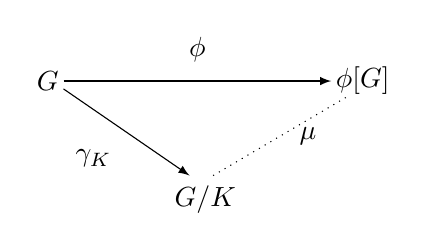
\begin{tikzpicture}
		\draw (0,1.5) node {$G$};
		\draw (2,0) node {$G/K$};
		\draw (4,1.5) node {$\phi[G]$};
		\draw[-latex] (0.2,1.4) -- node(e1)[sloped,label=below:$\gamma_K$]{} (1.8,0.3);
		\draw[-latex] (0.2,1.5) -- node(e2)[label=above:$\phi$]{} (3.6,1.5);
		\draw[dotted] (2.1,0.3) -- node(e2)[label=right:$\mu$]{} (3.8,1.3);
	\end{tikzpicture}
	\caption{First Isomorphism Theorem}
\end{figure}

\subsection{Second Isomorphism Theorem}
\begin{definition}

	Join $H \vee N$ is the smallest subgroup of $G$ containing $HN$ where $HN = \{ hn : h \in H, n \in N\}$.
\end{definition}

\begin{lemma}
	Let $N$ be a normal subgroup of $G$ and let $\gamma : G \to G/N$ be the canonical homomorphism.
	Then the map $\phi$ from the set of normal subgroups of $G$ containing $N$ to the set of normal subgroup of $G/N$ given by $\phi(L) = \gamma[L]$ is one-to-one and onto.
\end{lemma}
\begin{proof}
	Let $G$ be a group and $N$ be a normal subgroup of $G$.
	Given that $\gamma : G \to G/N$ the canonical homomorphism.
	That is, $\gamma(g) = gN$ for every $g \in G$.
	Let $L,M$ be normal subgroups of $G$ containing $N$.
	Since homomorphism preserves normality, $\gamma(L)$ is a normal subgroup of $\gamma[G]$.

	Suppose $\phi(L) = \phi(M)$.
	By definition of $\phi$,
	\begin{equation*}
		\gamma[L] = \phi(L) = \phi(M) = \gamma[M]
	\end{equation*}
	Since $N$ is normal, $\gamma^{-1}(\gamma(g)) = gN$ for every $g \in G$.
	And
	\begin{equation*}
		\gamma^{-1}(\gamma[L]) = \gamma^{-1} \left( \bigcup_{g \in L} \gamma(g) \right) = \bigcup_{g \in L} \gamma^{-1}(\gamma(g)) = \bigcup_{g \in L} gN = L
	\end{equation*}
	for every point $g \in L$, the left coset $gN$ is contained in $L$. ($\because N \subgroup L$)
	Therefore,
	\begin{equation*}
		\gamma^{-1} (\phi(L))  = \gamma^{-1} (\gamma[L]) = L 
	\end{equation*}
	\begin{equation*}
		\gamma^{-1} (\phi(M)) = \gamma^{-1} (\gamma[M]) = M
	\end{equation*}
	Thus, $L = M$.
	Therefore, $\phi$ is injective.

	Let $H$ be a normal subgroup of $G/N$.
	Then $\gamma^{-1}(H)$ is a normal subgroup of $G$.
	We have, $eN \in H$ and $\gamma^{-1}(eN) = eN = N$.
	Thus, $N \subset \gamma^{-1}(H)$.
	Thus, there exists $\gamma^{-1}(H)$, a normal subgroup of $G$ containing $N$ such that $\phi(\gamma^{-1}(H)) = H$.
	Therefore, $\phi$ is surjective.
\end{proof}

\begin{lemma}
	If $N$ is a normal subgroup of $G$, then $H \cap N = HN = NH$.
	Furthermore, if $H$ is also normal in $G$, then $HN$ is normal in $G$.
\end{lemma}
\begin{proof}
	Let $G$ be a group and $N$ be a normal subgroup of $G$.
	Also let $H$ be a subgroup of $G$.\\
	Claim : $HN = \{ hn \in G : h \in H,\ n \in N \}$ is a subgroup of $G$.
	\begin{enumerate}[label=G\arabic*]
		\item Closure : $h_1n_1h_2n_2 = h_1(h_2n_3)n_2 = h_3n_4 \in HN$, where $h_1,h_2 \in H$ and $n_1,n_2,n_4 \in N$. Since $N$ is normal, $n_1h_2 = h_2n_3$ for some $n_3 \in N$.
		\item $HN \subset G$, thus $HN$ satisfies associativity.
		\item Since $H,N \subgroup G$, $e \in H$ and $e \in N$. Thus, $e = ee \in HN$.
		\item Let $h_1n_1 \in HN$. $H \subgroup G$ and $h_1 \in H \implies h_1^{-1} \in H$. Then $n_1^{-1}h_1^{-1} = h_1^{-1}n_2$ for some $n_2 \in N$, since $N$ is normal. Thus, every element in $HN$, $h_1n_1$ has an inverse $h_1^{-1}n_2 \in HN$.
	\end{enumerate}
	Let $H$ be a normal subgroup of $G$.
	Let $g \in G$.
	Then $g(h_1n_1) = (gh_1)n_1 = (h_2g)n_1 = h_2(gn_1) = h_2(n_2g) = (h_2n_2)g$ for some $h_2 \in H$ and $n_2 \in N$ since both $H$ and $N$ are normal subgrops of $G$.
	Thus $gHN = HNg$ for every $g \in G$.
	Therefore, $HN$ is a normal subgroup of $G$.
\end{proof}

\begin{theorem}[second isomorphism]
	Let $H$ be a subgroup of $G$ and let $N$ be a normal subgroup of $G$.
	Then $(HN)/N \isomorphism H/(H\cap N)$.
\end{theorem}
\begin{proof}
	\begin{figure}
		\centering
		\begin{tikzpicture}
			\draw[-latex] (2,2) --node[above]{$\gamma_{|_{HN}}$} (6,2);
			\draw[-latex] (2,2) -- (4,0);
			\draw[dotted] (6,2) --node[left]{$\mu_1$} (4,0);
			\draw[-latex] (10,2) --node[above]{$\gamma_{|_H}$} (6,2);
			\draw[-latex] (10,2) -- (8,0);
			\draw[dotted] (8,0) --node[right]{$\mu_2$} (6,2);
			\draw[dotted] (8,0) --node[above]{$\mu_1 \circ \mu_2^{-1}$} (4,0);
			\draw (1,2) node{$HN$};
			\draw (6,2.5) node{$\gamma[H]$};
			\draw (10.5,2) node{$H$};
			\draw (4,-0.5) node{$HN/N$};
			\draw (8,-0.5) node{$H/H\cap N$};
		\end{tikzpicture}
		\caption{Second Isomorphism Theorem}
	\end{figure}
	Consider the canonical homomorphism $\gamma : G \to G/N$ with kernel $N$.
	Then $\gamma$ restricted to $HN$ is a homomorphism from $HN$ onto $\gamma[H]$.
	\begin{equation}
		\gamma_{|_{HN}} : HN \to \gamma[H] \text{ where } \gamma_{|_{HN}}(hn) = \gamma(hn) = (hn)N = hN = \gamma(h)
	\end{equation}
	Since $\ker(\gamma) = N$ and $N \subset HN$. We have, $\ker(\gamma_{|_{HN}}) = N$. 
	By first isomorphism therorem there exists a unique isomorphism $\mu_1 : HN/N \to \gamma[H]$ where $\mu_1(hnN) = \gamma(h) = hN$.\\

	Similarly, $\gamma$ restricted to $H$ is also a homomorphism onto $\gamma[H]$.
	\begin{equation}
		\gamma_{|_H} : H \to \gamma[H] \text{ where } \gamma_{|_H}(h) = \gamma(h) = hN.
	\end{equation}
	Since $\ker(\gamma) = N$ and $H \cap N \ne \phi$. $\ker(\gamma_{|_H}) = H \cap N$. By first isomorphism theorem, there exists a unique isomorphism $\mu_2 : H/(H\cap N) \to \gamma[H]$% where $\mu_2(h(H \cap N)) = \gamma(h) = hN$.\\

	Then $HN/N \isomorphism H/(H \cap N)$, since the composition of two isomorphisms, $\mu_2^{-1}\circ \mu_1 : HN/N \to H/(H \cap N)$ is an isomorphism% where $\mu_2^{-1}\circ \mu_1 (hnN) = \mu_2^{-1} (\gamma(h)) = \mu_2^{-1} (hN) = h(H \cap N)$.
\end{proof}

%Week 5 Day 2 \S34.6-10
\section{Third Isomorphism Theorem}
\begin{theorem}[third isomorphism]
	Let $H$ and $K$ be normal subgroup of $G$ with $K \le H$.
	Then $G/H \isomorphism (G/K)/(H/K)$.
\end{theorem}
\begin{proof}
\begin{figure}[h]
	\centering
	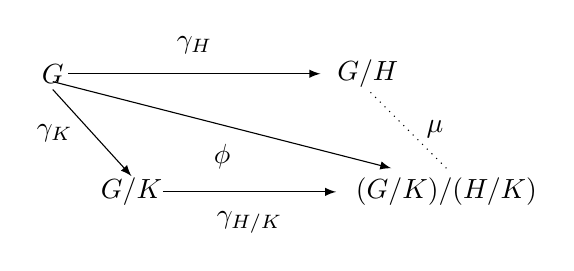
\begin{tikzpicture}
		\draw (0,1.5) node {$G$};
		\draw (1,0) node {$G/K$};
		\draw (5,0) node {$(G/K)/(H/K)$};
		\draw (4,1.5) node {$G/H$};
		\draw[-latex] (0,1.3) -- node(e1)[label=left:$\gamma_K$]{} (1,0.2);
		\draw[-latex] (0.2,1.5) -- node(e2)[label=above:$\gamma_H$]{} (3.4,1.5);
		\draw[-latex] (1.4,0) -- node(e3)[label=below:$\gamma_{H/K}$]{} (3.6,0);
		\draw[-latex] (0,1.4) -- node(e4)[label=below:$\phi$]{} (4.3,0.3);
		\draw[dotted] (5,0.3) -- node(e5)[label=right:$\mu$]{} (4,1.3);
	\end{tikzpicture}
	\caption{Third Isomorphism Theorem}
\end{figure}
	Consider the function $\phi : G \to (G/K)/(H/K)$ defined by $\phi(g) = gK(H/K)$.
	Then, $\phi$ is a homomorphism.
	\begin{align*}
		\phi(ab) & = (ab)K/(H/K) \\
		& = (aK)(bK)\ (H/K),\ \because (ab)K = (aK)(bK) \\
		& = aK(H/K)\ bK(H/K),\ \because (xy)H/K = xH/K\ yH/K\\
		& = \phi(a) \phi(b)
	\end{align*}
	The kernel of $\phi$ is the set $\{ a \in G : \phi(a) = H/K \}$.
	Since the coset $H/K$ was originally the points in $H$, we have $\ker(\phi) = H$.
	By first isomorphism theorem, there exists a unique isomorphism $\mu : G/H \to (G/K)/(H/K)$. Thus, $G/H \isomorphism (G/K)/(H/K)$.
\end{proof}

%Week 6 Day 1-2 \S36.1-7
\section{Finite, non-abelian Groups}
\begin{theorem}
	Let $p$ be a prime. Let $G$ be a group of order $p^n$.
	Let $X$ be a finite $G$-set.
	Then $|X| \equiv |X_G| \pmod{p}$.
\end{theorem}
\begin{proof}
	Suppose there are $r$ orbits in $X$.
	Choose an element from each orbit, say $x_1,x_2,\cdots,x_r$.
	We have, 
	\begin{equation}
		|X| = \sum_{i = 1}^r |Gx_i|
	\end{equation}
	Let $X_G = \{ x \in X : gx = x,\ \forall g \in G \}$.
	Then each element in $X_G$ belongs to an orbit of length 1.
	Let $|X_G| = s$. Then,
	\begin{equation}
		|X| = |X_G| + \sum_{i = s+1}^r |Gx_i|
	\end{equation}
	We have, $|Gx| = (G:G_x)$.
	Clearly, both $G$ and $G_x$ are groups of order a multiple of prime $p$.
	Thus, for every $x \in X$, $|Gx|$ is multiple of prime $p$.
	Therefore, $|X| \cong |X_G| \pmod{p}$.
\end{proof}

\begin{challenge}
	Let $p$ be a prime and $G$ be a finite group $G$.
	Design a mechanism to enumerate all elements of order $p$ ?
\end{challenge}

\begin{definition}
	Let $G$ be a group. Let $p$ be a prime. $G$ is a \textbf{$p$-group} if every element of $G$ has order a power of $p$.
	A subgroup $H$ of $G$ is a \textbf{$p$-subgroup} of $G$ if every element of $H$ has order a power of $p$.
\end{definition}
\begin{theorem}[Cauchy]
	Let $p$ be a prime.
	Let $G$ be a finite group and $p$ divides $|G|$, then $G$ has a subgroup of order $p$.
\end{theorem}
\begin{proof}
	Let $X$ be the set of all $n$-tuples of elements of $G$ such that the product of co-ordinates of each $n$-tuple is the identity element $e$ of $G$.
	\begin{equation}
	X = \{ (g_1,g_2,\cdots,g_p) \in G^p : g_1g_2\cdots g_p = e\}
	\end{equation}
	Let $g_1,g_2,\cdots,g_{p-1}$ be any elements in $G$.
	Then $g_p = (g_1g_2\cdots g_{p-1})^{-1}$ is uniquely determined.
	That is, the $(p-1)$ co-ordinates of an element in $X$ may be chosen in $|G|$ different ways.
	Thus, $|X| = |G|^{p-1}$.
	Since $p$ divides $|G|$, $p$ divides $|X|$.

	We have $g_1(g_2\cdots g_p) = (g_2g_3\cdots g_p)g_1$, since $g_2g_3\cdots g_p = g_1^{-1}$.
	Thus, for every $(g_1,g_2,\cdots,g_p) \in X$, the $\sigma$ permutation of that element is in $X$.
	That is, $\sigma(g_1,g_2,\cdots,g_p) = (g_2,g_3,\cdots,g_p,g_1) \in X$.
	Similarly, $g_2(g_3g_4\cdots g_pg_1) = (g_3g_4\cdots g_pg_1)g_2$.
	And $\sigma^2(g_1,g_2,\cdots,g_p) = g_3,g_4,\cdots,g_p,g_1,g_2)$.
	Clearly, the subgroup generated by $\sigma$, is a subgroup of $S_p$ and $X$ is a $<\!\sigma\!>$-set.
	We have, $|X| \cong |X_{<\sigma>}| \pmod{p}$.
	Thus, $p$ divides $|X_{<\sigma>}|$.

	Clearly, $(e,e,\cdots,e) \in X$ and $(e,e,\cdots,e) \in X_{<\sigma>}$.
	Thus, $X_{<\sigma>}$ has atleast $p$ elements.
	Let $(g_1,g_2,\cdots,g_p) \in X_{<\sigma>}$, then $\sigma$ fixes $(g_1,g_2,\cdots,g_p)$.
	\begin{align*}
		\sigma(g_1,g_2,\cdots,g_p) & = (g_1,g_2,\cdots,g_p)\\
		\implies (g_2,\cdots,g_p,g_1) & = (g_1,g_2,\cdots,g_p)
	\end{align*}
	Thus, $g_1 = g_2 = \cdots = g_p$, say $g \in G$.
	That $(g,g,\cdots,g) \in X$ and $g^p = e$ by the definition of $X$.
	Therefore, $G$ has an element $g$ of order $p$.
\end{proof}
\begin{corollary}
	Let $G$ be a finite group. Then $G$ is a $p$-group if and only if $|G|$ is a power of $p$.
\end{corollary}
\begin{proof}
	Let $G$ be a finite group.
	Suppose $G$ is a $p$-group.
	Suppose there exists another prime $q$, $q \ne p$ such that $q$ divides $|G|$.
	Then by Cauchy's theorem, $G$ has an element of order $q$.
	This contradicts the assumption that $G$ is a $p$-group.
	Thus, the only prime that divides $|G|$ is $p$.
	Therefore, the order of $G$ is a power of prime $p$.

	Let $|G|=p^n$.
	Then the factors of $p^n$ are powers of $p$.
	By Lagrange's theorem, order of subgroups of $G$ must divide $|G|$.
	Thus, every subgroup of $G$ has order a power of $p$.
	Thus, every element of $G$ has order a power of $p$.
	Therefore, $G$ is a $p$-group.
\end{proof}

\begin{definition}
	Let $G$ be a group and $H$ be a subgroup of $G$.
	Consider the inner automorphisms $i_g : G \to G$ such that $i_g(x) = gxg^{-1}$.
	We have, $i_g(H) = gHg^{-1}$ is the conjugate of the subgroup $H$.
	The set of all elements in $G$ which has $H$ itself as the conjugate of $H$ is the normaliser of $H$ in $G$.
	\begin{equation}
		N[H] = \{ g \in G : gHg^{-1} = H\}
	\end{equation}
\end{definition}

\begin{remark}
	The normaliser of $H$ in $G$ is a subgroup of $G$.
	And $N[H]$ is the largest subgroup of $G$ with $H$ as its normal subgroup.
\end{remark}
\begin{lemma}
	Let $H$ be a $p$-subgroup of a finite group $G$. Then
	\begin{equation}
		(N[H] : H) \cong (G:H) \pmod{p}
	\end{equation}
\end{lemma}
\begin{proof}
	Let $G$ be a finite group.
	Let $H$ be a $p$-subgroup of $G$.
	Let $\mathscr{L}$ be the set of all left cosets of $H$ in $G$.
	Then, $|\mathscr{L}| = (G:H)$.

	Claim : $\mathscr{L}$ is an $H$-set with group action $h(xH) = (hx)H$.
	We have, $e(xH) = (ex)H = xH$ and $(g_1g_2)(xH) = (g_1g_2xH) = g_1(g_2xH) = g_1(g_2(xH))$.

	Let $\mathscr{L}_H$ be the set of all left cosets that are fixed under action by all element of $H$.
	\begin{align*}
		\mathscr{L}_H & = \{ xH \in \mathscr{L} : h(xH) = xH,\ \forall h \in H\} \\
		& = \{ xH \in \mathscr{L} : x^{-1}h (xH) = H,\ \forall h \in H \} \\
		& = \{ xH \in \mathscr{L} : (x^{-1}hx)H = H,\ \forall h \in H \} \\
		& = \{ xH \in \mathscr{L} : (x^{-1}hx) \in H,\ \forall h \in H \} \\
		& = \{ xH \in \mathscr{L} : x^{-1} \in N[H] \}
	\end{align*}
	Clearly, left cosets of $\mathscr{L}_H$ has all its elements contained in $N[H]$. Thus,
	\begin{equation}
		|\mathscr{L}_H| = (N[H]:H)
	\end{equation}
	We have, $\mathscr{L}$ is an $H$-set.
	And $H$ is a $p$-subgroup.
	Thus, $H$ has order a power of prime $p$.
	Therefore, 
	\begin{equation}
		|\mathscr{L}| \cong |\mathscr{L}_H| \pmod{p}
	\end{equation}
\end{proof}

\begin{corollary}
	Let $H$ be a $p$-subgroup of finite group $G$.
	If $p$ divides $(G:H)$, then $N[H] \ne H$.
\end{corollary}
\begin{proof}
	We have, $(G:H) \cong (N[H]:H) \pmod {p}$.
	And $p$ divides $(G:H)$.
	Thus, $p$ divides $(N[H]:H)$.
	Therefore, $H \ne N[H]$.
\end{proof}

%Week 6 Day 3 \S36.8-13
\section{Sylow Theorems}
\begin{theorem}[First Sylow Theorem]
	Let $G$ be a finite group of order $p^n m$ where $n \ge 1$ and $p$ does not divide $m$. Then
	\begin{enumerate}
		\item $G$ contains a subgroup of order $p^i$ where $1 \le i \le n$.
		\item Every subgroup $H$ of $G$ of order $p^i$ is normal subgroup of the subgroup of order $p^{i+1}$, for $1 \le i \le n$.
	\end{enumerate}
%	For each prime factor $p$ of $|G|$, there exists a subnormal series\footnote{Fraleigh, uses series instead of sequence in \S35.1!} of $G$.
%	That is, $H_0 \le H_1 \le \cdots \le H_n = G$.
\end{theorem}
\begin{proof}
	We have, $G$ is finite group and $p$ divides $|G|$.
	By Cauchy's theorem, $G$ has a subgroup of order $p$.

	Suppose $G$ has a subgroup $H$ of order $p^i$, where $(i < n)$.
	Then, $H$ is a $p$-subgroup.
	Thus, $(G:H) \cong (N[H]:H) \pmod{p}$ where $N[H]$ is the normaliser of $H$ in $G$.
	Clearly, $p$ divides $(G:H)$.
	Thus, $p$ divides $(N[H]:H)$.

	And $H$ is a normal subgroup of $N[H]$.
	Thus, we have factor group $N[H]/H$ and $p$ divides the order of $N[H]/H$.
	By Cauchy's theorem, $N[H]/H$ has a subgroup $K$ of order $p$.
	Consider the canonical homomorphism $\gamma : N[H] \to N[H]/H$ defined by $\gamma(x) = xH$.
	Then $\gamma^{-1}(K)$ is a subgroup of $N[H]$ of order $p^{i+1}$ and contains $H$.
	Thus, $H$ is a normal subgroup of $\gamma^{-1}(K)$.
	By mathematical induction, $G$ has subgroups of order $p^i$ for $i = 2,3,\cdots,n$.
\end{proof}

\begin{definition}
	A sylow $p$-subgroup of $G$ is a maximal $p$-subgroup of $G$.
\end{definition}

\begin{theorem}[Second Sylow Theorem]
	Let $P_1$ and $P_2$ be two Sylow $p$-subgroups of $G$.
	Then $P_1$ and $P_2$ are conjugate subgroups of $G$.
\end{theorem}
\begin{proof}
	Let $P_1$ and $P_2$ be two Sylow $p$-subgroups of $G$.
	Let $\mathscr{L}$ be the set of all left cosets of $P_1$.
	Then, group $P_2$ act on $\mathscr{L}$ by $y(xP_1) = (yx)P_1$.
	Thus, $\mathscr{L}$ is a $P_2$-set.
	Therefore, $|\mathscr{L}| \cong |\mathscr{L}_{P_2}| \pmod{p}$.

	Clearly $|\mathscr{L}| = (G:P_1)$.
	And $p$ doesn't divide $|\mathscr{L}|$.
	Thus, $p$ does not divide $|\mathscr{L}_{P_2}|$.
	Therefore, $|\mathscr{L}_{P_2}| > 0$.

	Thus, $\mathscr{L}$ has at least an element $xP_1$ which is fixed in the action of every element in $P_2$.
	That is, $yxP_1 = xP_1$ for every $y \in P_2$.
	Therefore, $x^{-1}yxP_1 = P_1$ for every $y \in P_2$.

	In other words, $x^{-1}yx \in P_1$ for every $y \in P_2$.
	Therefore, $x^{-1}P_2x \subgroup P_1$.
	But, $|P_1| = |P_2|$.
	Thus, $x^{-1}P_2x = P_1$.
	Therefore, $P_1$ and $P_2$ are conjugate subgroups of $G$.
\end{proof}


\begin{theorem}[Third Sylow Theorem]
	If $G$ is a finite group and $p$ divides $|G|$, then the number of Sylow $p$-subgroups is congruent to $1 \pmod{p}$ and divides $|G|$.
\end{theorem}
\begin{proof}
	Let $\mathscr{S}$ be the set of all Sylow $p$-subgroups of $G$.
	Let $P$ be a Sylow $p$-subgroup of $G$.
	The elements of $P$ act on $\mathscr{S}$ by conjugation.
	Let $x \in P$ and $T \in \mathscr{S}$, then $x$ carries $T$ into $xTx^{-1}$.
	Clearly, $\mathscr{S}$ is a $P$-set.

	We have, $|\mathscr{S}| \cong |\mathscr{S}_P| \pmod{p}$.
	Suppose $T \in \mathscr{S}_P$.
	Then, $xTx^{-1} = T$ for every $x \in P$.
	Thus, $T$ is a normal subgroup of $P$.
	But, $T$ and $P$ are of the same order, since both are Sylow $p$-subgroups of $G$.	
	Therefore, $T = P$.
	Thus, $\mathscr{S}_P = \{ P \}$.
	And $|\mathscr{S}_P| = 1$.
	Thus, $|\mathscr{S}| \cong 1 \pmod{p}$.

	Let $G$ act of $\mathscr{S}$ by conjugation.
	Let $x \in G$ and $P \in \mathscr{S}$, then $x$ carries $P$ into $xPx^{-1}$.
	Clearly, $\mathscr{S}$ is a $G$-set.
	However, every Sylow $p$-subgroup of $G$ are conjugates.
	Thus, thus every Sylow $p$-subgroup of $G$ belong to the same orbit under conjugation action.
	We have, $|Gx| = (G:G_x)$ and thus length of orbits divides the order of $G$.
	Since the number of Sylow $p$-subgroups is same as the length of the orbit of $P$, the number of Sylow $p$-subgroup of $G$ divides the order of $G$.
\end{proof}

\begin{remark}
	Let $G$ be a group of order $15$.
	Let $p = 3$.
	By Third Sylow Theorem, the number of Sylow $3$-subgroup of $G$ is congruent to $1 \pmod{3}$ and divides $15$.
	We have, congruence class $\hat{1} = \{ 1,4,7,10,13 \}$.
	Only $1$ divides $15$.
	Thus, there is only one Sylow $3$-subgroup of $G$.

	Let $p = 5$.
	By Third Sylow Theorem, the number of Sylow $5$-subgroup of $G$ is congruent to $1 \pmod{5}$ and divides $15$.
	We have, congruence class $\hat{1} = \{ 1,6,11 \}$.
	Only $1$ divides $15$.
	Thus, there is only one Sylow $3$-subgroup of $G$.
\end{remark}

\begin{remark}
	Let $G$ be a group of order $255$.
	And $1,3,5,15,17,51,85,255$ are the divisors of $255$.
	Let $p = 3$.
	By third Sylow theorem, either there is one or eighty-five Sylow $3$-subgroups of $G$.
	Suppose there $85$ Sylow $3$-subgroups. Then there are $170$ elements of order $3$.
	
	Let $p = 5$.
	By third Sylow theorem, either there are one or fifty-one Sylow $5$-subgroups of $G$.	
	Suppose there $51$ Sylow $5$-subgroups. Then there are $204$ elements of order $5$.

	Let $p = 17$.
	By third Sylow theorem, there is exactly one Sylow $17$-subgroup of $G$.	Thus, there are exactly $16$ elements of order $17$ in $G$.
\end{remark}

%Week 7 Day 1 \S37.1-6
\section{Sylow Theorem : Applications}
\begin{definition}
	A group $G$ is solvable if there is sequence of subgroups $\{e\} = H_0 \le H_1 \le \cdots H_n = G$ such that for $i = 0,1,2,\cdots$,
	\begin{enumerate}
		\item $H_i$ is a normal subgroup of $H_{i+1}$
		\item $H_{i+1}/H_i$ is simple and
		\item $H_{i+1}/H_i$ is abelian.
	\end{enumerate}
\end{definition}

\begin{theorem}
	Every group of prime order is solvable.
\end{theorem}
\begin{proof}
\end{proof}

\begin{definition}
	Let $G$ be a finite group.
	Consider $G$ acting on itself by conjugation. Then,
	\begin{equation}|G| = |Z(G)| + \sum_{s+1}^r |Gx_i|
	\end{equation}
	This is the class equation of $G$.
	And each orbit of $G$ under conjugation by itself is a conjugate class in $G$.
\end{definition}

\begin{theorem}
	The center of a finite, nontrivial $p$-group is nontrivial.
\end{theorem}
\begin{proof}
\end{proof}

\begin{lemma}
	Let $G$ be a group containing normal subgroups $H$ and $K$ such that $H \cap K = \{e\}$ and $H \vee K = G$.
	Then $G$ is isomorphic to $H \times K$.
\end{lemma}
\begin{proof}
\end{proof}

\begin{theorem}
	For a prime number $p$, every group of $G$ of order $p^2$ is abelian.
\end{theorem}
\begin{proof}
\end{proof}
